

\subsection{Combining statistical evidence}

The first general category of methods for genomic data integration
consists of approaches where evidence across similar studies is
combined to increase statistical power, for instance by comparing and
integrating data from independent microarray experiments targeted at
studying the same disease. In Publications~\ref{RPA} and~\ref{NR},
joint analysis of a large number of commensurable microarray
experiments, where the observed data is directly comparable between
the arrays, helps to increase statistical power and to reveal weak,
shared signals in the data that can not be detected in more restricted
experimental setups and smaller datasets. 

However, the related observations are often not directly comparable,
and further methodological tools are needed for integration. {\it
Meta-analysis} provides tools for such analysis
\citep{Ramasamy08b}. Meta-analysis forms part of the microarray
analysis procedure introduced in Publication~\ref{PECA}, where methods
to integrate related microarray measurements across different array
platforms are developed. Meta-analysis emphasizes shared effects
between the studies over statistical significance in individual
experiments. In its standard form, meta-analysis assumes that each
individual study measures the same target variable with varying levels
of noise. The analysis starts from identifying a measure of {\it
effect size} based on differences, means, or other summary statistics
of the observations such as the Hedges' g, used in
Publication~\ref{PECA}. Weighted averaging of the effect sizes
provides the final, combined result. Weighting accounts for
differences in reliability of the individual studies, for instance by
emphasizing studies with large sample size, or low measurement
variance. Averaging is expected to yield more accurate estimates of
the target variable than individual studies. This can be particularly
useful when several studies with small sample sizes are available for
instance from different laboratories, which is a common setting in
microarray analysis context, where the data sets produced by
individual laboratories are routinely deposited to shared community
databases. Ultimately, the quality of meta-analysis results rests on
the quality of the individual studies. Modeling choices, such as the
choice of the effect size measure and included studies will affect the
analysis outcome.

{\it Kernel methods} \citep[see e.g.][]{Scholkopf02} provide another
widely used approach for integrating statistical evidence across
multiple, potentially heterogeneous measurement sources. Kernel
methods operate on similarity matrices, and provide a natural
framework for combining statistical evidence to detect similarity and
patterns that are supported by multiple observations. The modeling
framework also allows for efficient modeling of nonlinear feature
spaces.

{\it Multi-task learning} refers to a class of approaches where
multiple, related modeling tasks are solved simultaneously by
combining statistical power across the related tasks. A typical task
is to improve the accuracy of individual classifiers by taking
advantage of the potential dependencies between them \citep[see
e.g.][]{Caruana97}.


\subsection{Role of side information}

The second category of approaches for genomic data integration
consists of methods that are asymmetric by nature; integration is used
to support the analysis of one, primary data source. Side information
can be used, for instance, to limit the search space and to focus the
analysis to avoid overfitting, speed up computation, as well as to
obtain potentially more sensitive and accurate findings \citep[see
e.g.][]{Eisenstein06}. One strategy is to impose hard constraints on
the model, or model family, based on side information to target
specific research questions. In gene expression context, functional
classifications or known interactions between the genes can be used to
constrain the analysis \citep{Goeman07, Ulitsky09}. In factor analysis
and mixed effect models, clinical annotations of the samples help to
focus the modeling on particular conditions \citep[see
e.g.][]{Carvalho08}. Hard constraints rely heavily on the accuracy of
side information. Soft, or probabilistic approaches can take the
uncertainty in side information into account, but they are
computationally more demanding. Examples of such methods in the
context of transcriptome analysis include for instance the supervised
biclustering models, such as cMonkey and modified SAMBA, as well as
other methods that guide the analysis with additional information of
genes and regulatory mechanisms, such as transcription factor binding
\citep{Reiss06, Savage2010, Tanay04}. Publication~\ref{NR} uses gene
interaction network as a hard constraint for modeling transcriptional
co-regulation of the genes, but the condition-specific responses of
the detected gene groups are identified in an unsupervised manner.

A complementary approach for utilizing side information of the
experiments is provided by {\it multi-way learning}. A classical
example is the analysis of variance (ANOVA), where a single data set
is modeled by decomposing it into a set of basic, underlying effects,
which characterize the data optimally. The effects are associated with
multiple, potentially overlapping attributes of the measurement
samples, such as disease state, gender and age, which are known prior
to the analysis. Taking such prior knowledge of systematic variation
between the samples into account helps to increase modeling power and
can reveal the attribute-specific effects. An interesting subtask is
to model the interactions between the attributes, so-called {\it
interaction effects}. These are manifested only with particular
combinations of attributes, and indicate dependency between the
attributes. For instance, simultaneous cigarette smoking and asbestos
exposure will considerably increase the risk of lung cancer, compared
to any of the two risk factors alone \citep[see
e.g.][]{Nymark07}. {\it Factor analysis} is a closely related approach
where the attributes, also called {\it factors}, are not given but
instead estimated from the data. {\it Mixed effect models} combine the
supervised and unsupervised approaches by incorporating both {\it
fixed} and {\it random effects} in the model, corresponding to the
known and latent attributes, respectively \citep[see
e.g.][]{Carvalho08}. The standard factorization approaches for
individual data sets are related to the dependency-seeking approaches
in Publications~\ref{MLSP}-\ref{AC}, where co-occurring data sources
are decomposed in an unsupervised manner into components that are
maximally informative of the components in the other data set. 

\subsection{Modeling of mutual dependency}

Symmetric models for dependency detection form the third main category
of methods for genomic data integration, as well as the main topic of
this chapter. Dependency modeling is used to distinguish the {\it
shared} signal from {\it dataset-specific} variation. The shared
effects are informative of the commonalities and interactions between
the observations, and are often the main focus of interest in
integrative analysis. This motivates the development of methods that
can allocate computational resources efficiently to modeling of the
shared features and interactions.

{\it Multi-view learning} is a general category of approaches for
symmetric dependency modeling tasks. In multi-view learning, multiple
measurement sources are available, and each source is considered as a
different view on the same objects. The task is to enhance modeling
performance by combining the complementary views. A classical example
of such a model is canonical correlation analysis
\citep{Hotelling36}. Related approaches that have recently been applied
in functional genomics include for instance probabilistic variants of
meta-analysis \citep{Choi07, Conlon07}, generalized singular value
decomposition \citep[see e.g.][]{Alter03, Berger06} and simultaneous
non-negative matrix factorization \citep{Badea08}.

The dependency modeling approaches in this thesis make an explicit
distinction between statistical representation of data and the
modeling task.  Let us denote the representations of two co-occurring
multivariate observations, $\x$ and $\y$, with $f_x(\x)$ and
$f_y(\y)$, respectively. The selected representations depend on the
application task. The representation can be for instance used to
perform feature selection as in {\it canonical correlation analysis
(CCA)} \citet{Hotelling36}, capture nonlinear features in the data as
in kernelized versions of CCA \citep[see e.g.][]{Yamanishi03}, or
partition the data as in information bottleneck \citep{Friedman01} and
associative clustering (Publications~\ref{ECML}-\ref{AC}). {\it
Statistical independence} of the representations implies that their
joint probability density can be decomposed as \(p(f_x(\x), f_y(\y)) =
p(f_x(\x))p(f_y(\y))\). Deviations from this assumption indicate
statistical dependency. The representations can have a flexible
parametric form which can be optimized by the dependency modeling
algorithms to identify dependency structure in the data.

Recent examples of such dependency-maximizing methods include
probabilistic canonical correlation analysis \citep{Bach05}, which has
close theoretical connection to the regularized models introduced in
Publication~\ref{MLSP}, and the associative clustering principle
introduced in Publications~\ref{ECML}-\ref{AC}. Canonical
correlations and contingency table analysis form the methodological
background for the contributions in Publications~\ref{MLSP}-\ref{AC}.
In the remainder of this section these two standard approaches for
dependency detection are considered more closely.

\subsubsection{Classical and probabilistic canonical correlation analysis}

Canonical correlation analysis (CCA) is a classical method for
detecting linear dependencies between two multivariate random
variables \citep{Hotelling36}. While ordinary correlation
characterizes the association strength between two vectors with paired
scalar observations, CCA assumes paired vectorial values, and
generalizes correlation to multidimensional sources by searching for
maximally correlating low-dimensional representation of the two
sources, defined by linear projections \(\X\vx, \Y\vy\). Multiple
projection components can be obtained iteratively, by finding the most
correlating projection first, and then consecutively the next ones
after removing the dependencies explained by the previous CCA
components; the lower-dimensional representations are defined by
projections to linear hyperplanes. The model can be formulated as a
generalized eigenvalue problem that has an analytical solution with
two useful properties: the result is invariant to linear
transformations of the data, and the solution for any fixed number of
components maximizes mutual information between the projections for
Gaussian data \citep{Kullback59, Bach02}. Extensions of the classical
CCA include generalizations to multiple data sources
\citep{Kettenring71, Bach02}, regularized solutions with non-negative
and sparse projections \citep{Sigg07, Archambeau08, Witten09}, and
non-linear extensions, for instance with kernel methods \citep{Bach02,
Yamanishi03}. Direct optimization of correlations in the classical CCA
provides an efficient way to detect dependencies between data sources,
but it lacks an explicit model to deal with the uncertainty in the
data and model parameters.

Recently, the classical CCA was shown to correspond to the ML solution
of a particular generative model where the two data sets are assumed
to stem from a shared Gaussian latent variable \(\z\) and normally
distributed data-set-specific noise \citep{Bach05}. Using linear
assumptions, the model is formally defined as

\begin{flalign}\label{eq:genmodel}
     \left\{
   \begin{array}{cl}
	\x &\sim \Wx \z + \Epsx\\
	\y &\sim \Wy \z + \Epsy.
  \end{array}
\right.
\end{flalign}

\noindent The manifestation of the shared signal in each data set can
be different. This is parameterized by \(\W_x\) and \(\W_y\).
Assuming a standard Gaussian model for the shared latent variable,
\(\z \sim \N(\0,\I)\) and data set-specific effects where \(\Epsx \sim
\N(\0, \Psi_x)\) (and respectively for \(\y\)), the
correlation-maximizing projections of the traditional CCA introduced
in Section~\ref{sec:traditionaldep} can be retrieved from the ML
solution of the model \citep{Archambeau06, Bach05}. The model
decomposes the observed co-occurring data sets into {\it shared} and
{\it data set-specific} components based on explicit modeling
assumptions (Figure~\ref{fig:modelpic}). The dataset-specific effects
can also be described in terms of latent variables as \(\Epsx =
\B_x\z_x\) and \(\Epsy = \B_y\z_y\), allowing the construction of more
detailed models for the dataset-specific effects \citep{Klami08}. The
shared signal \(\z\) is treated as a latent variable and marginalized
out in the model, providing the marginal likelihood for the
observations:

\begin{equation}\label{eq:ccalikelihood}
    p(\X,\Y|\W,\Psi) = \int p(\X, \Y|\Z, \W, \Psi)p(\Z) d\Z,
\end{equation}

\noindent where \(\Psi\) denotes the block-diagonal matrix of
\(\Psi_x\), \(\Psi_y\), and \(\W = [\W_x; \W_y]\).  The probabilistic
formulation of CCA has opened up a way to new probabilistic extensions
that can treat the modeling assumptions and uncertainties in the data
in a more explicit and robust manner \citep{Archambeau06, Klami08,
Klami10uai}.

The general formulation provides a flexible modeling framework, where
different modeling assumptions can be used to adapt the models in
different applications. The connection to classical CCA assumes full
covariances for the dataset-specific effects. Simpler models for the
dataset-specific effects will not distinguish between the shared and
marginal effects as effectively, but they have fewer model parameters
that can potentially reduce overlearning and speed up computation.  It
is also possible to tune the dimensionality of the shared latent
signal. Learning of lower-dimensional models can be faster and
potentially less prone to overfitting. Interpretation of simpler
models is also more straightforward in many applications. The
probabilistic formulation allows rigorous treatment of uncertainties
in the data and model parameters also with small sample sizes that are
common in biomedical studies, and allows the incorporation of prior
information through Bayesian priors, as in the regularized dependency
detection framework introduced in Publication~\ref{MLSP}.


\begin{figure}[ht!]
\centering{ 
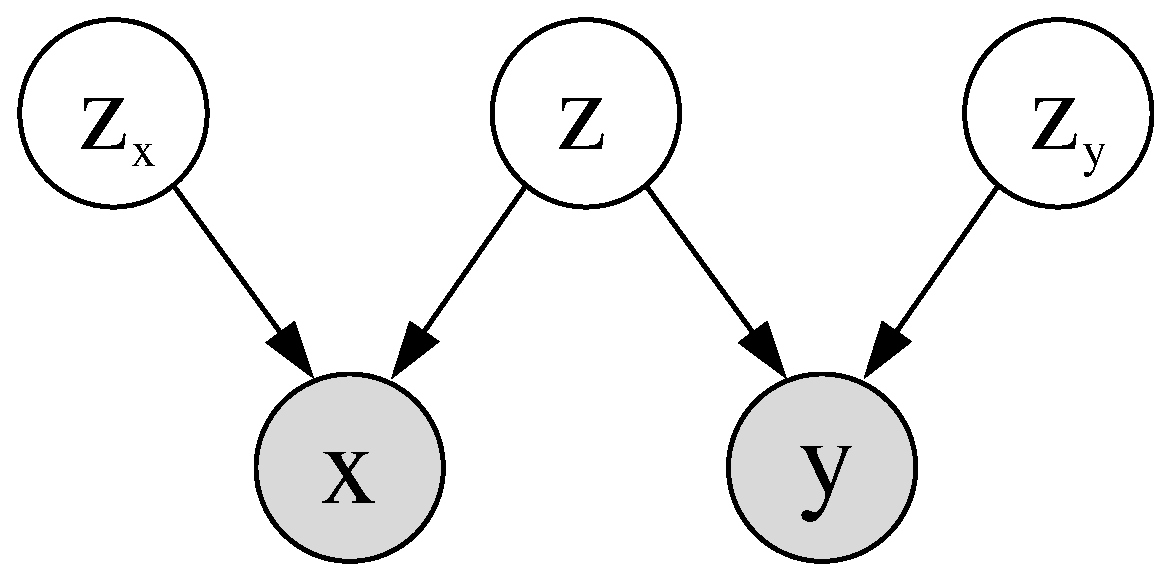
\includegraphics[width=.4\textwidth]{pic/depmodel.eps}
}
\caption{A graphical representation of the generative shared latent
  variable model in Equation~(\ref{eq:genmodel}). The latent source
  $\z$ is shared by observations $\x$ and $\y$. The other effects that
  are specific to each observation are characterized by $\z_x$ and
  $\z_y$, respectively. Gray shading indicates observed variables.}
\label{fig:modelpic}
\end{figure}


\subsubsection{Contingency table analysis}

Contingency table analysis is a classical approach used to study
associations between co-occurring categorical observations.  The
co-occurrences are represented by cross-tabulating them on a {\it
contingency table}, the rows and columns of which correspond to the
first and second set of features, respectively. Various tests are
available for measuring dependency between the rows and columns of the
table \citet{Yates34, Agresti92}, including the classical Fisher test
\citep{Fisher34}, a standard tool for measuring statistical enrichment
of functional categories in gene cluster analysis
\citep{Hosack03}. While the classical contingency table analysis is
used to measure dependency between co-occurring variables, more recent
approaches use contingency tables to derive objective functions for
dependency exploration tasks. The associative clustering principle
introduced in Publications~\ref{ECML}-\ref{AC} is an example of such
approach.

Other approaches that use contingency table dependencies as objective
functions include the {\it information bottleneck (IB)} principle
\citep{Tishby99} and {\it discriminative clustering (DC)}
\citep{Sinkkonen02ecml, Kaski05nc}. These are asymmetric,
dependency-seeking approaches that can be used to discover cluster
structure in a primary data such that it is maximally informative of
another, discrete auxiliary variable. The dependency is represented on
a contingency table, and maximization of contingency table
dependencies provides the objective function for clustering. While the
standard IB operates on discrete data, DC is used to discover cluster
structure in continuous-valued data. The two approaches also employ
different objective functions. In classical IB, a discrete variable
$\Xcal$ is clustered in such a way that the cluster assignments become
maximally informative of another discrete variable $\Ycal$. The
complexity of the cluster assignments is controlled by minimizing the
mutual information between the cluster indices and the original
variables. The task is to find a partitioning $\tilde{\X}$ that
minimizes the cost \(\L(p(\tilde{\X}|\X)) = I(\tilde{\X}; \X) - \beta
I(\tilde{\X}; \Y),\) where $\beta$ controls clustering resolution. In
DC, mutual information is replaced by a Bayes factor between the two
hypotheses of dependent and independent margins. The Bayes factor is
asymptotically consistent with mutual information, but provides an
unbiased estimate for limited sample size \citep[see
e.g.][]{Sinkkonen05tr}. The standard information bottleneck and
discriminative clustering are asymmetric methods that treat one of the
data sources as the primary target of analysis.

In contrast, the dependency maximization approaches considered in this
thesis, the associative clustering (AC) and regularized versions of
canonical correlation analysis are symmetric and they operate
exclusively on continuous-valued data.  CCA is not based on
contingency table analysis, but it has close connections to the
Gaussian IB \citep{Chechik05} that seeks maximal dependency between
two sets of normally distributed variables. The Gaussian IB retrieves
the same subspace as CCA for one of the data sets. However, in
contrast to the symmetric CCA model, Gaussian IB is a directed method
that finds dependency-maximizing projections for only one of the two
data sets.  The second dependency detection approach considered in
this thesis, the associative clustering, is particularly related to
the symmetric IB that finds two sets of clusters, one for each
variable, which are optimally compressed presentations of the original
data, and at the same time maximally informative of each other
\citep{Friedman01}. While the objective function in IB is derived from
mutual information, AC uses the Bayes factor as an objective function
in a similar manner as it is used in the asymmetric discriminative
clustering. Another key difference is that while the symmetric IB
operates on discrete data, AC employs contingency table analysis in
order to discover cluster structure in continuous-valued data spaces.






